%----------------------------------------------------------------------------
\chapter{Tervezési kritériumok meghatározása}
\label{sec:Tervezesi_kriteriumok}
%----------------------------------------------------------------------------

A diploma dolgozatomban, ahogy a bevezetőben is említettem egy telemanipulátor geometriai, elektronikai és szoftveres tervezését, ezeknek az elemeknek az elkészítését és működését fogom bemutatni. Az első lépés a felsorolt feladatok teljesítéséhez, hogy egy átfogó szempontrendszert hozzak létre. Ez abban segített nekem, hogy a tervezési lépéseknél figyelembe véve az produktum így egységes és a meghatározott funkciókkal van ellátva.  

\section{Telemanipulátorokról általánosan}
%----------------------------------------------------------------------------

Fogalmi tisztázásképpen szeretném előbb bemutatni, hogy általános megfogalmazásban mi a telemanipulátor. Ez egy olyan eszközöket magába foglaló robotikai rendszer, amely lehetővé teszi egy operátor\footnote{Egy személy, aki a mozgás utasítások kiadását közvetlenül végzi} számára, hogy közvetve irányítson és mozgásutasításokat adjon egy robotkarnak vagy manipulátornak. Az ilyen típusú rendszerek jellemzően két jól elhatárolható részből állnak, egy vezérlőpanelből (továbbiakban HMI - Human Machine Interface) és egy fizikai manipulátorból, amellyel a mozgásutasítás cél pozícióját vagy orientációját lehet megadni a robotkarnak vagy manipulátoroknak.

A telemanipulátoros rendszerek célja, hogy a valós robot mozgatás és a operátor pozíciója helyben ne legyen korlátozva. Lehetővé tegye azt, hogy a robotkar vagy manipulátor közvetlen vezérlését biztonságosabb, nyugodtabb vagy - az én általam elkészített telemanipulátor esetében - egy szoftveres réteg mögül tegye meg. A telemanipulátorok fő alkalmazási területe, ahol szükséges az, hogy az operátor és a robotkar térben független lehessen egymástól. Ezek az eszközök széles körben alkalmazhatók különböző iparágakban és területeken, például az űrkutatásban és az űrtörmelék, vagy minta gyűjtésben. Az orvostudományban a telemanipulátorok segítségével végezhetnek távoli műtéteket és beavatkozásokat. Az ipar területén például a gyártásban használják ezeket a megoldásokat nehezen programozható pályák megvalósítására, vagy nagyfokú precizitást igénylő munkafolyamatok elvégzésére.

Az alkalmazási területtől függ, hogy mennyire terjedelmes, de az általánosan megállapítható, hogy egy telemanipulátor rendszernek számos elvárásnak kell megfelelnie, hogy biztonságosan tudjuk alkalmazni. A geometriától indulva ergonomikusnak kell lennie, mivel közvetlenül az operátor keze által vannak a mozgatási parancsok kiadva. Önmagában a telemanipulátor kezelése gondot okoz, akkor a mozgatás se lesz kielégítő. A szoftveres rendszernek a sebessége a másik kritérium, hogy a rendszernek az adott mozgásutasítás és a tényleges mozgás között minimális legyen az eltérés. Ez két általánosan megfogalmazott elvárást, önmagában a tervezési lépéseknél figyelembe lehet és kell venni.

A telemanipulátor rendszerek különböző szenzorokat (erő, távolság vagy szögállás) vagy mozgás detektáló rendszereket (képfeldolgozás) használnak, hogy pontos vezérlést biztosítsanak az operátor számára. A folyamatosan fejlődő technológiák, például a virtuális valóság és a vezetéknélküli rendszerek, további lehetőségeket kínálnak a telemanipulátorok alkalmazásának területén.

Összességében a telemanipulátor rendszerek lehetővé teszik az ember és a robot együttműködését, és hozzájárulnak a térben korlátok nélküli, "távoli" helyeken történő feladatok hatékony és biztonságos elvégzéséhez. Ezáltal a telemanipulátorok alkalmazása előnyös lehet olyan helyzetekben, ahol emberi jelenlét nem kívánatos vagy nem lehetséges, de mégis szükség van az emberi kézügyességre és irányításra.

\section{Szakdolgozatomban elkészített telemanipulátor}
%----------------------------------------------------------------------------

A tervezési elvárások meghatározásának alapja az alapszintű képzésem Szakdolgozatában dokumentált hat szabadsági fokú telemanipulátor. Az eszköz tervezése volt az első önálló mérnöki munkám, amelynek eredményeképpen sikerült egy átfogó projektet bemutatnom. Ez a telemanipulátor egy egyszerű egytagú karokból és csuklókból összeállított kinematikai eszköz. Az eszköz elkészítésének koncepciója az volt, hogy a hatodik csuklóba helyezhető legyen egy tetszőleges geometria, amelynek a Tool Center Point (rövidítve TCP)\footnote{Tool Center point, ami egy definiált pontja az end-effektornak egy viszonyítási koordináta rendszerben.}-jának térben való elmozdulását mérni tudjam a karok egymáshoz viszonyított csuklószögeinek mérésével. Az \ref{fig:Szakdoga_csipeszes}.ábrán az elkészült eszköz látható.\cite{szakdoga}

\begin{figure}[!ht]
\centering
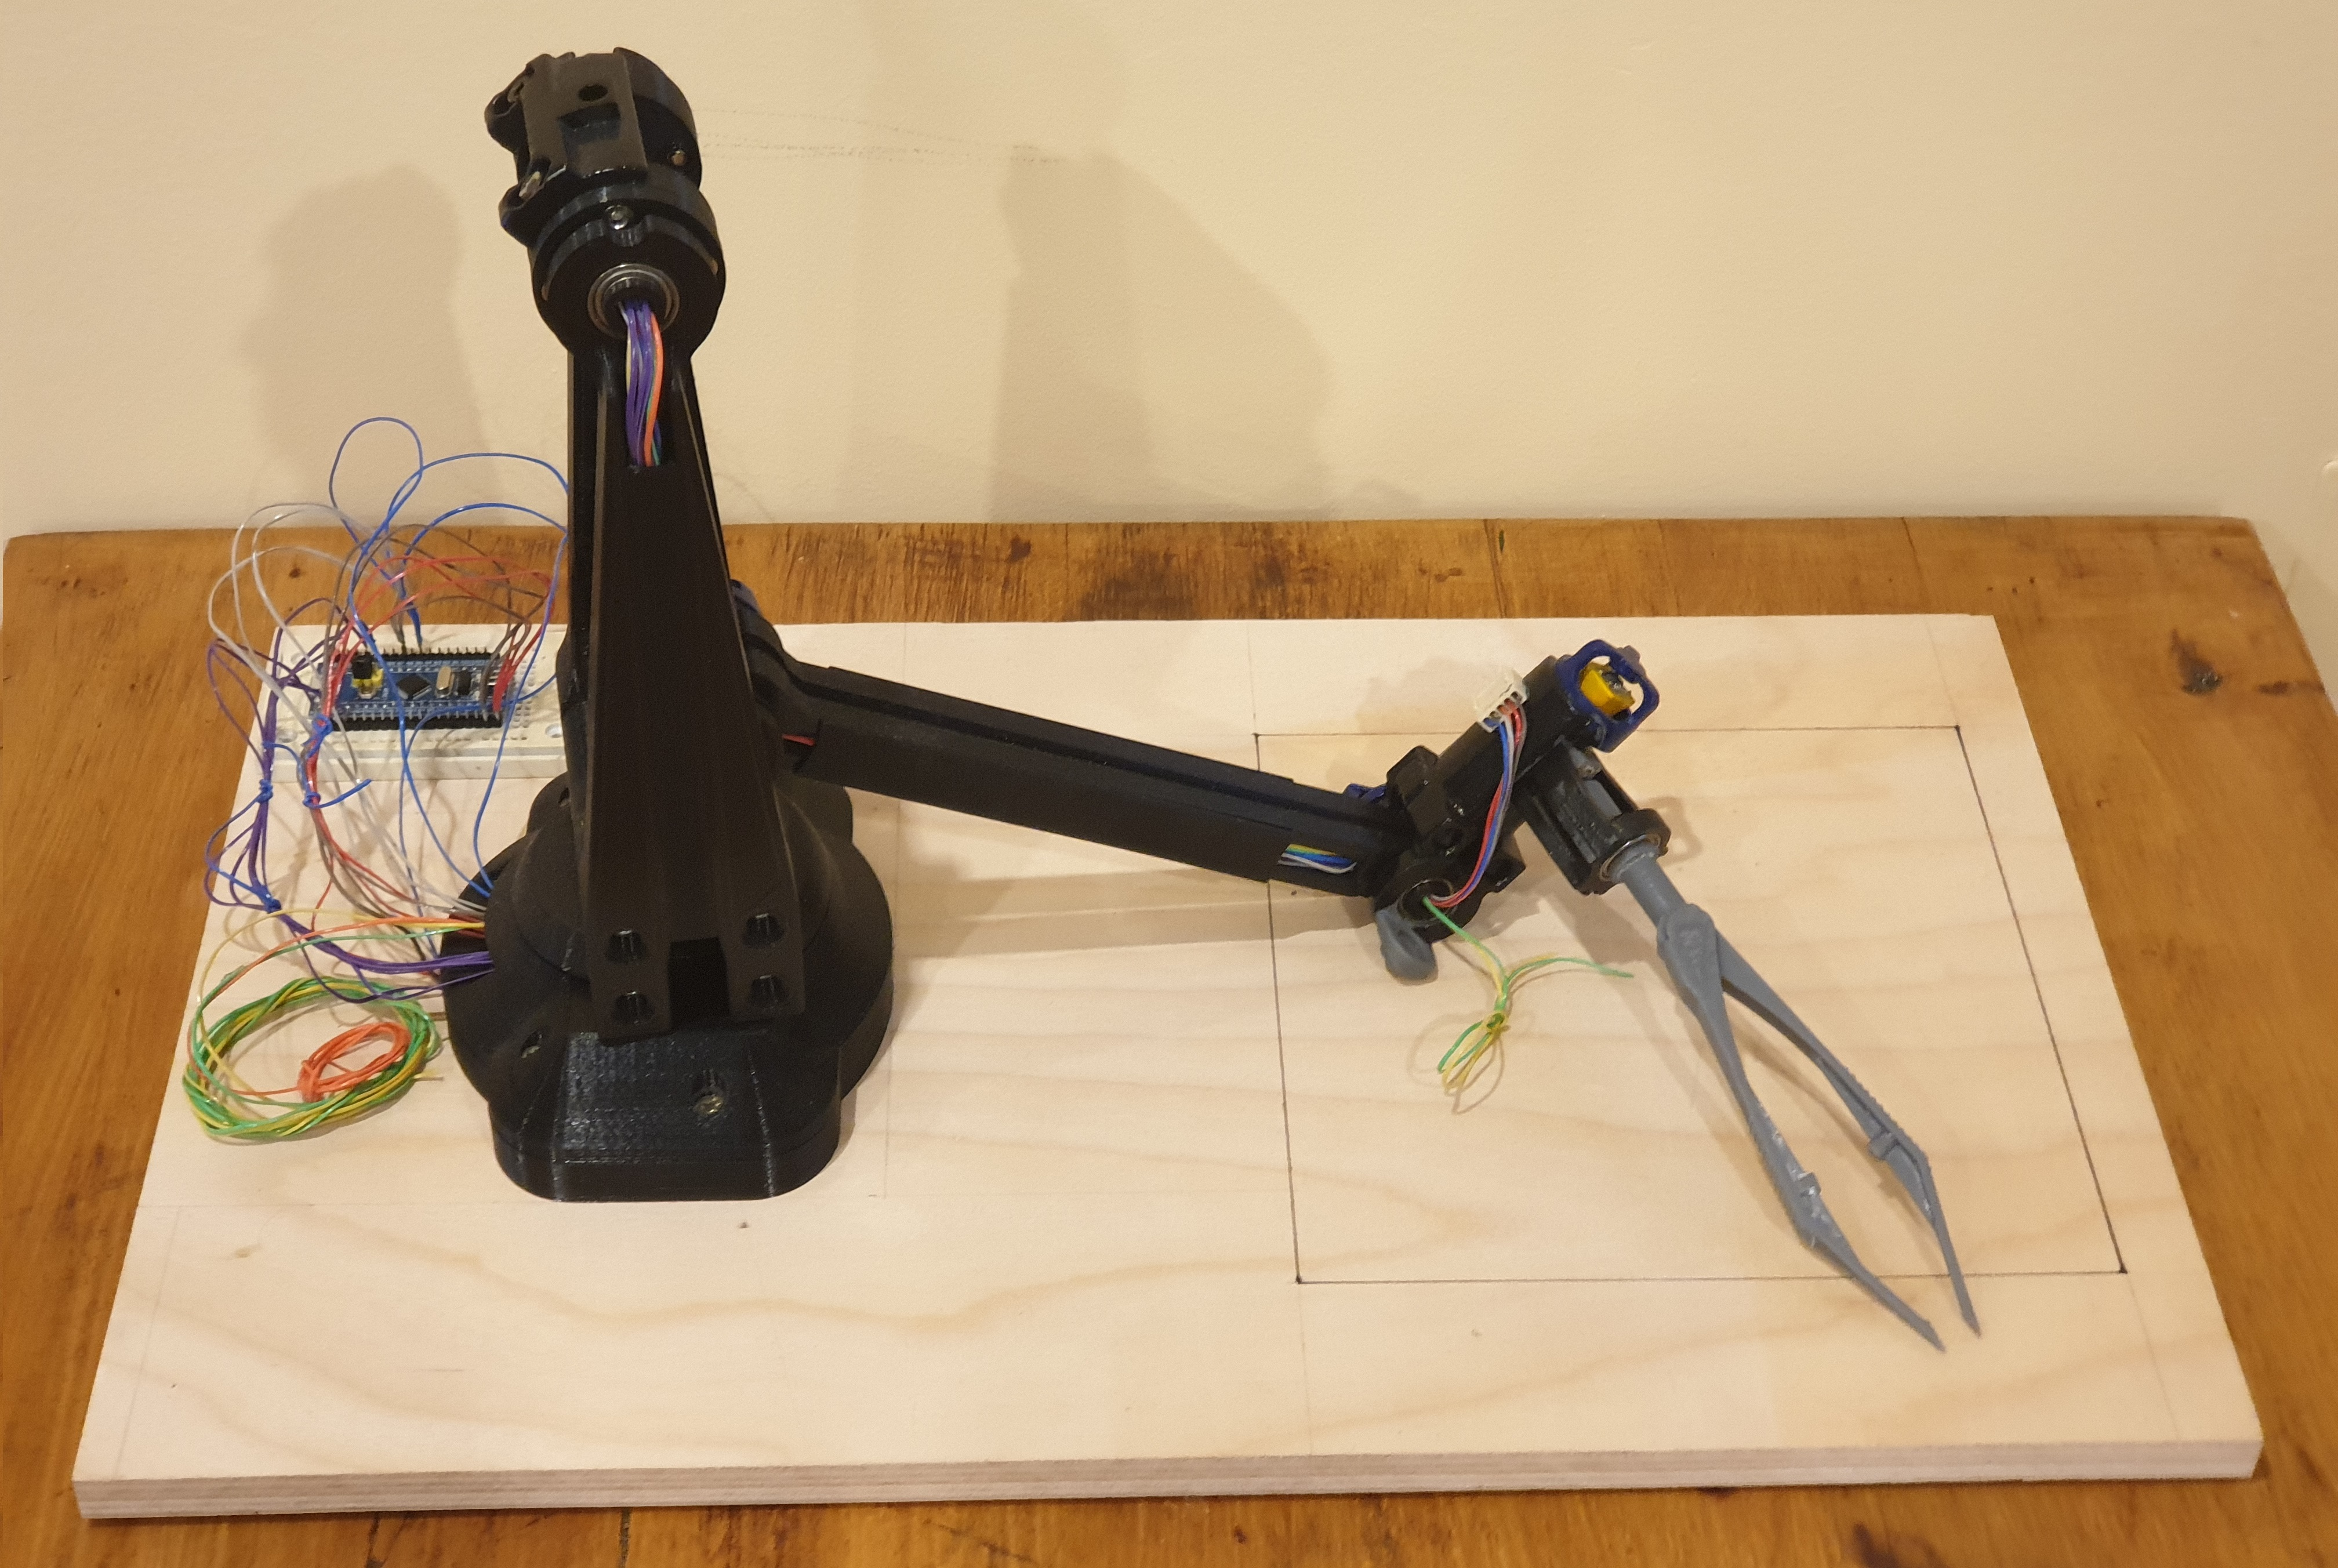
\includegraphics[width=120mm, keepaspectratio]{figures/Szakdoga/0_v_4_csipeszes}
\caption{Szakdolgozatomban elkészített telemanipulátor\cite{szakdoga}}
\label{fig:Szakdoga_telemanip_csipeszes}
\end{figure}

A telemanipulátort 3D nyomtatással lett készítettem el. Ez a prototípus készítési módszer manapság már a mérnöki munka alapjának tekinthető, főleg az megfizethető 3D nyomtató berendezések elterjedésével. Az általam használt nyomtatási technológia az alkatrészek nyomtatására ebben az esetben FDM\footnote{Fused Deposition Modeling - A nyomtatási technológia a hőre lágyuló polimerekkel képes 3D-s objektumokat nyomtatni. Az FDM nyomtatók azzal az alapelvvel működnek, hogy szobahőmérsékleten szilárd hőre lágyuló polimert 180$^{\circ}$- 300$^{\circ}$C-ra melegítve ömledék állapotba kerülnek és a kívánt helyre lehet juttatni lineáris vezetékrendszer segítségével.\cite{noorani20173d}}, viszont néhány alkatrész, mint például a szenzortartók elkészítéséhez SLA\footnote{StereoLithography Apparatus - modellteret UV aktív gyantával tölti fel. A nyomtatási térben egy síklapra építi fel a tárgyat úgy, hogy az belemerül egy gyantával teli kádba, ahol a megfelelő rétegvastagságú folyékony gyanta réteget UV lézerrel térhálósítja és köti adhézióval az előző réteghez\cite{noorani20173d}} technológiai alapon működő nyomtatót használtam. \cite{szakdoga}

A telemanipulátor karok csatlakozásánál mindenhol csapágyakat használtam, ezzel biztosítva az egytengelyűséget és az ellenállás mentes elfordulást. A vezetékezésben igyekeztem mindenhol tengelyen átlépő vezetékpályát tervezni, ami nem akadályozza a rendszer mozgatását.\cite{szakdoga}

A mikrovezérlővel begyűjtött szögértékeket továbbítottam egy szimulációs rendszernek, amiben igyekeztem megfelelő számításokkal egy virtuális robotkart mozgatni. Végeredményben az adatokkal végzett számításokat nem sikerült maradéktalanul hibamentesen elvégezni. A szakdolgozat megírásának pillanatában nem voltam kellően felkészülve kinematikai számítások terén. Egy hibás egyenlet rendszert írtam fel, aminek az eredményeként a kiszámított koordináták amiket a robotnak követnie kellett volna helytelenek voltak. Ezt később a Mesterképzésemen projekt feladatom kapcsán korrigáltam.\cite{szakdoga}

\begin{figure}[!ht]
\centering
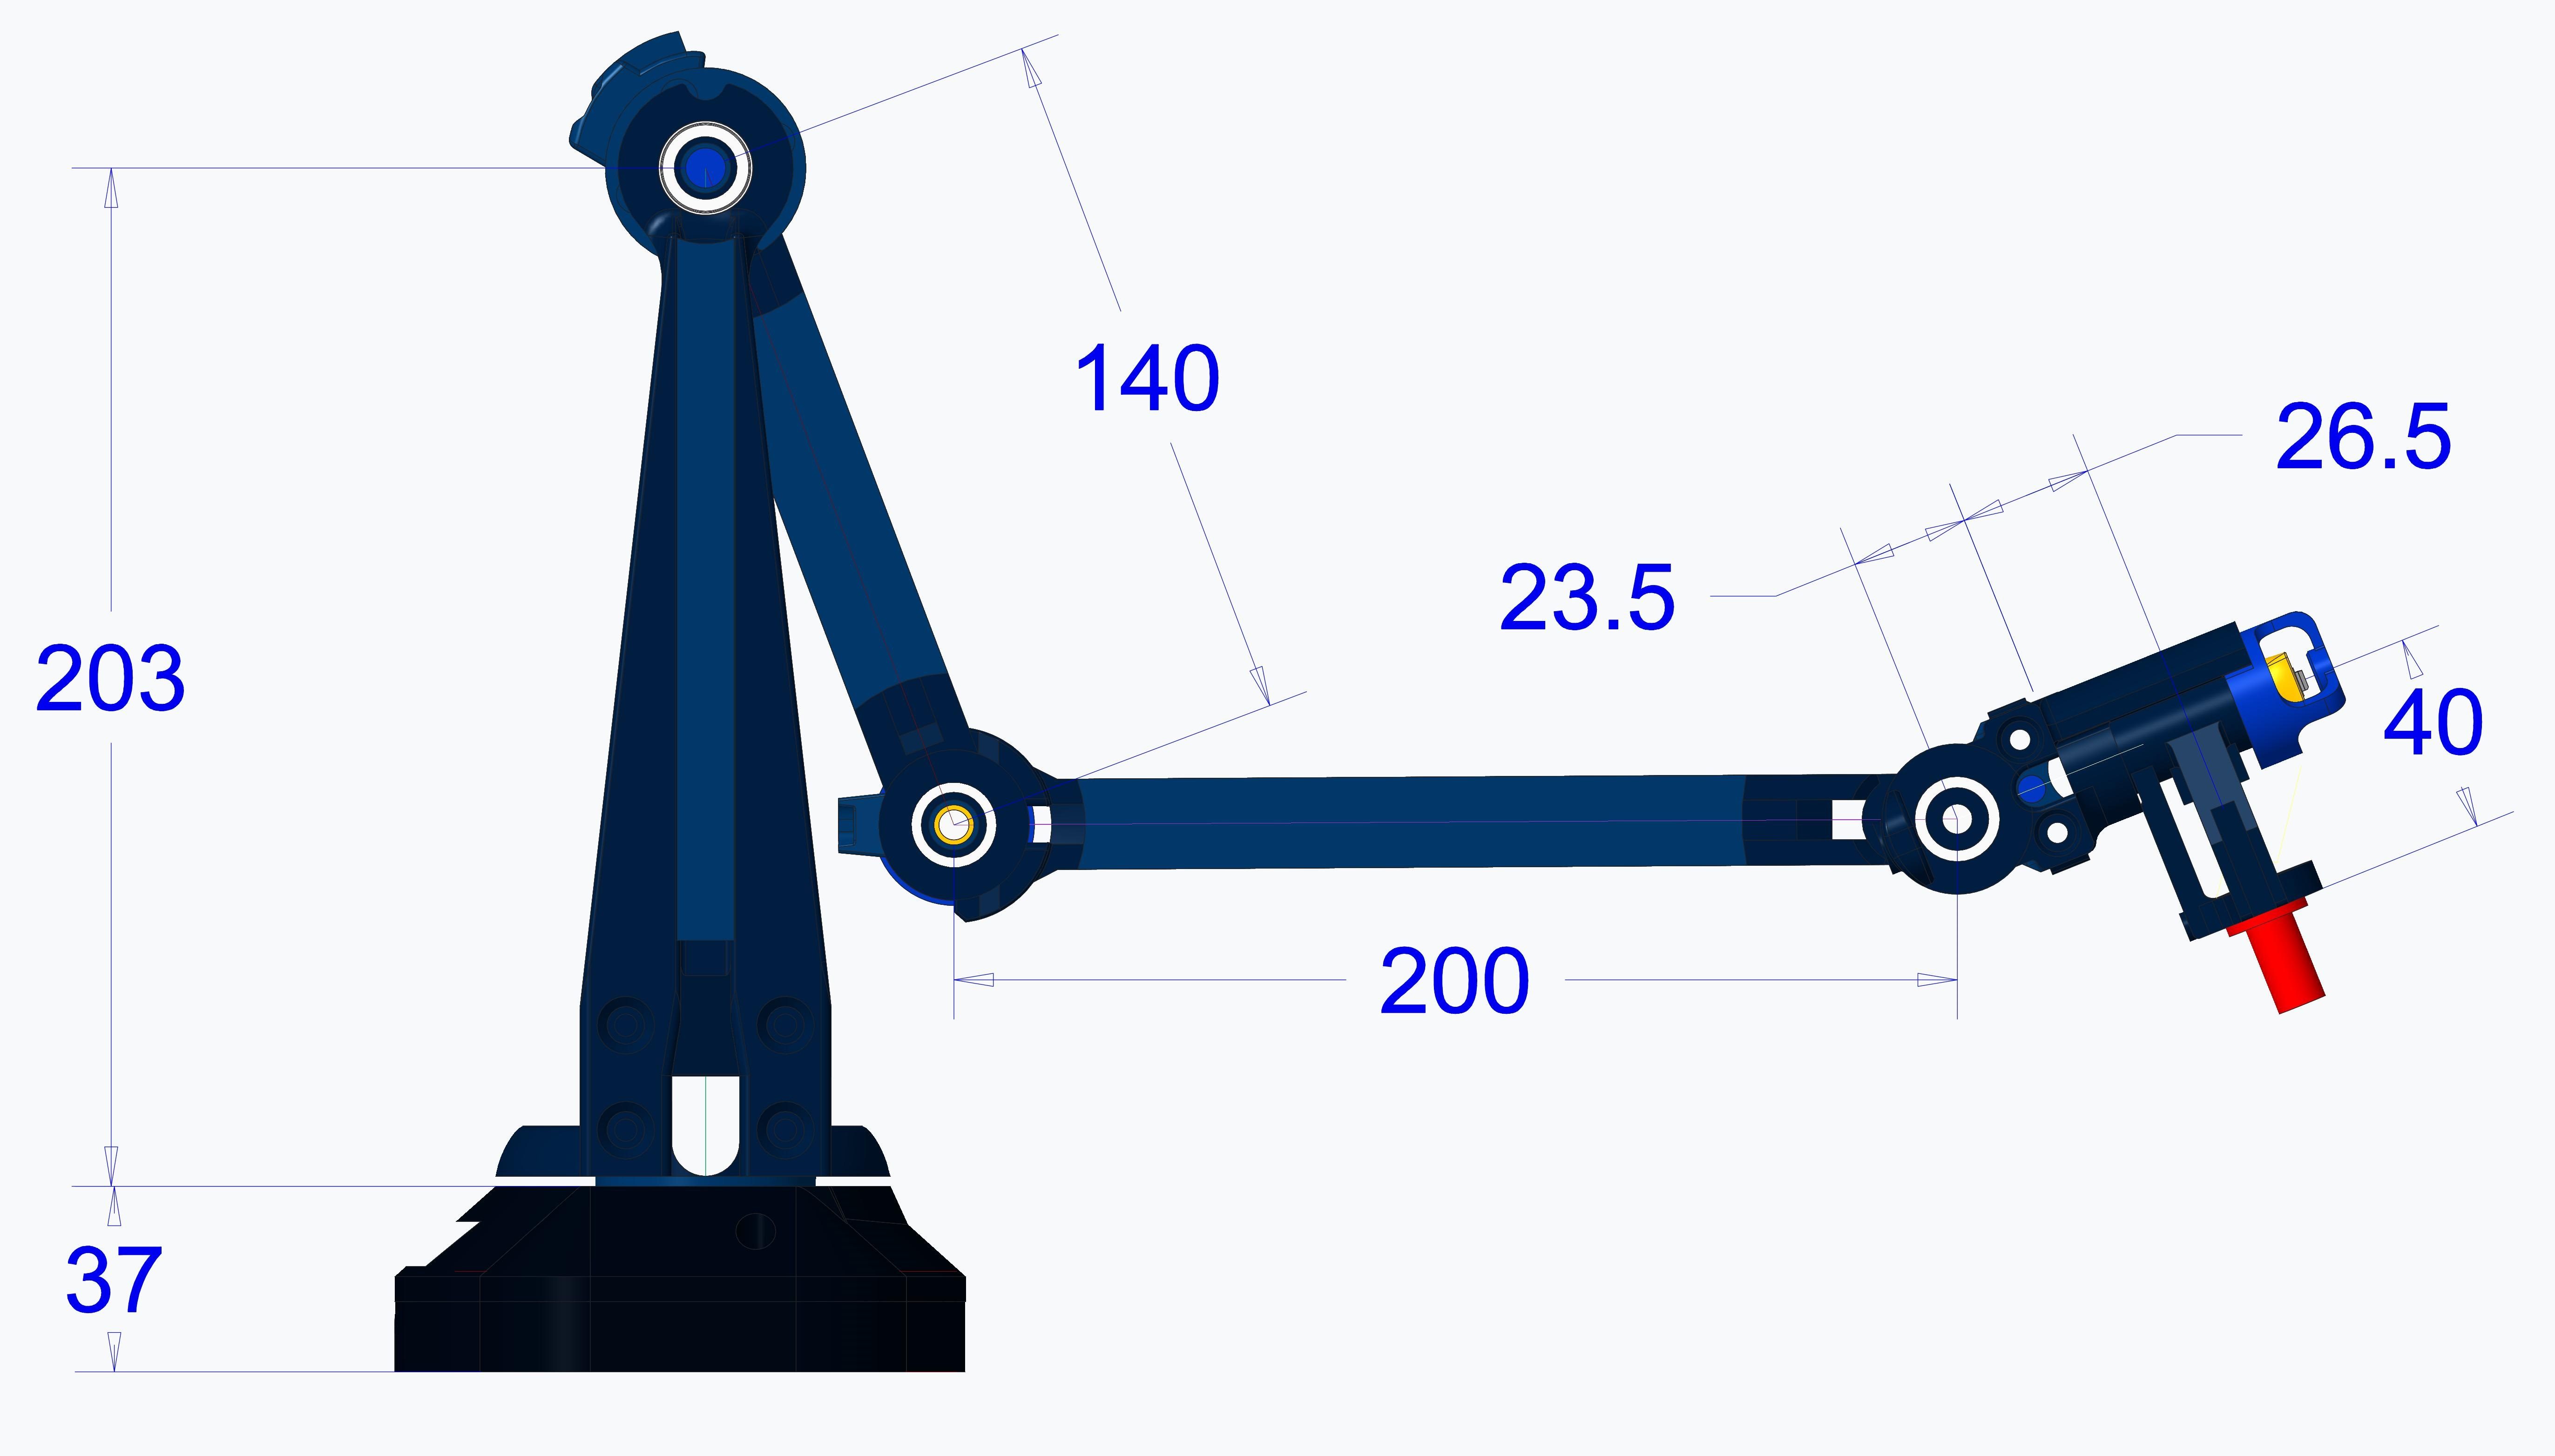
\includegraphics[width=120mm, keepaspectratio]{figures/Szakdoga/00_v_4_kar}
\caption{Szakdolgozatomban elkészített telemanipulátor méreteinek bemutatása\cite{szakdoga}}
\label{fig:Szakdoga_telemanip_meret}
\end{figure}

Végeredményben a szakdolgozatomban elkészített telemanipulátor az akkor meghatározott elvárásoknak tökéletesen megfelelt, viszont sok helyen koncepcionális és egy igen komoly számítási hibát tartalmazott. Mesterképzésemen az itt felmerülő hibákat céloztam meg első körben kijavítani. A munka közben megfogalmazott és a diplomamunkám elkészítéshez szükséges elvárásokat a következő fejezetben bemutatom.

\section{Újratervezési szempontok}
\label{sec:ujratervezesi_szempontok}
%----------------------------------------------------------------------------

A szakdolgozatomban az újratervezési szempontokat csoportosítás nélkül fogalmaztam meg, ami kissé általánosított megfogalmazást eredményezett. Az elvárások pontosan a következők voltak:

\begin{enumerate}
\item A manipulátor minél többféle eszköznek a rögzítését és mozgatását tegye lehetővé\cite{szakdoga}
\item Az eszközök a munkatere: $200[mm]x200[mm]x200[mm]$ \cite{szakdoga}
\item Az end-effektorra illesztett szerszámok használatát ne nehezítse a manipulátor súlya\cite{szakdoga}
\item Az eszköz geometriáját úgy kell kialakítani, hogy 3D nyomtatási technológiákkal legyártható legyen\cite{szakdoga}
\item A csuklóknál csapágyazást kell alkalmazni\cite{szakdoga}
\item Az eszköz kábelezését minél inkább el kell rejteni\cite{szakdoga}
\end{enumerate}

A diploma dolgozatom esetében is fontosnak éreztem ilyen pontokat megfogalmazni, de ezt csoportosítva teszem meg a következő alfejezetek alapján. A szakdolgozatban megtervezett és részletesen bemutatott telemanipulátor számomra legnagyobb hibája, hogy minden értelemben túl kicsi. Méretet és tömeget általában utolsóként szokás racionalizálni. Nincs elég hely az esetleges új funkcióknak és ha az egyik szenzor meghibásodik vagy másikat kell felhelyezni szinte a teljes eszközt újra kell kábelezni. Programozási tekintettben már az említett hiba mellett a mikrovezérlő memóriájában extra tárhely nincs, így itt se lehetséges az új funkciók implementálása. Így sokkal célzottabban lehetséges vizsgálni már a különböző problémákat a későbbiekben. Ezt követően egy funkcionális módosítást mutatok be, mielőtt a következő fejezetben a már új telemanipulátor tervezési lépéseit tárgyalnám.

\subsection{Geometriai újratervezési szempontok}

Az előző telemanipulátor karjainak méretei a kényelmes használat ellenére is túl rövidnek érződtek. A munkatér széle közelében már majdnem végállásban tudtak állni a karok, ezért ezeket mindenképpen nagyobbakra kell tervezni.

A kábel csatorna volt a legnagyobb gond. Ezt ugyan egy alapos számítással a kábelek száma és vastagsága alapján választottam meg, de pont emiatt új kábel behúzása nehezen vagy egyáltalán nem kivitelezhető. Az új karok esetében semmilyen formában nem szerettem volna kompromisszumos megoldást ezen a fronton, úgyhogy a megtervezett kar keresztmetszetének több mint $80\%$-át kábelcsatornává kellett alakítani.

Másik nagy munkát és újragondolást igénylő terület az ellensúlyos gravitációs hatásából származó terhelés kompenzációja, amiről a következő fejezetben részletesen kitérek. A szakdolgozatomnál az összes csukló esetében ezt szerettem volna megvalósítani, de ez korántsem lett a leghatékonyabb.

\subsection{Jelfeldolgozó rendszer újratervezési szempontok}

A jelfeldolgozó rendszer újratervezésére nem volt szükség. A szakdolgozatom bírálatában megfogalmazott bypass kondenzátor használatának lehetőségét viszont megvizsgáltam és megfogadtam. Így új szenzorokat készítettem kiegészítve ezzel a komponenssel. A mikrovezérlőnél viszont a perifériák száma és a memória mérete kevésnek bizonyult, így ezen a területen egy más, nagyobb kapacitású mikrovezérlő kiválasztását tűztem ki célul.

\subsection{Szoftveres újratervezési szempontok}

A jelfeldolgozó rendszertől kapott csuklószögeket felhasználó programmal szemben a legfontosabb elvárás, hogy hosszú távon valósidejű lefutást támogatni tudjon. Ez azért fontos, mert a KUKA robot kollaboratív robotjainak vezérléséhez ez elő követelmény.

A korábban említett számítási hiba kijavítása egyértelmű cél volt a szakdolgozatomat alapul véve, de ezt nem közvetlenül a diplomamunkám keretein belül végeztem el.

\newpage
\subsection{Sebészeti eszközök vezérlése}
%----------------------------------------------------------------------------

Röviden szeretnék kitérni arra, hogy a szakdolgozatomban látható ténylegesen modellezett sebészeti eszközöket a diploma dolgozatom esetében nem készítettem el. A cél ugyanaz, hogy egy olyan rendszert hozzak létre, ami sebészeti eszközök mozgatását tegye lehetővé robotkarok végén, viszont a rendszer elkészítéséhez nem szükséges már a tesztelésénél ezt használni. A szakdolgozatban látható telemanipulátor végén a csipesz és a szike modell megnehezítette a koordináták ellenőrzését. Emiatt azt detektálni nehéz volt, hogy mi következik szöghibákból és mi az egyedi end-effektor nem tökéletes ergonómiájából. Az sem elhanyagolható, hogy a dolgozatban a sebészeti eszköz tökéletesítése szerintem önmagában ki tudna tölteni egy teljes diplomamunkát.

\begin{figure}[!ht]
\centering
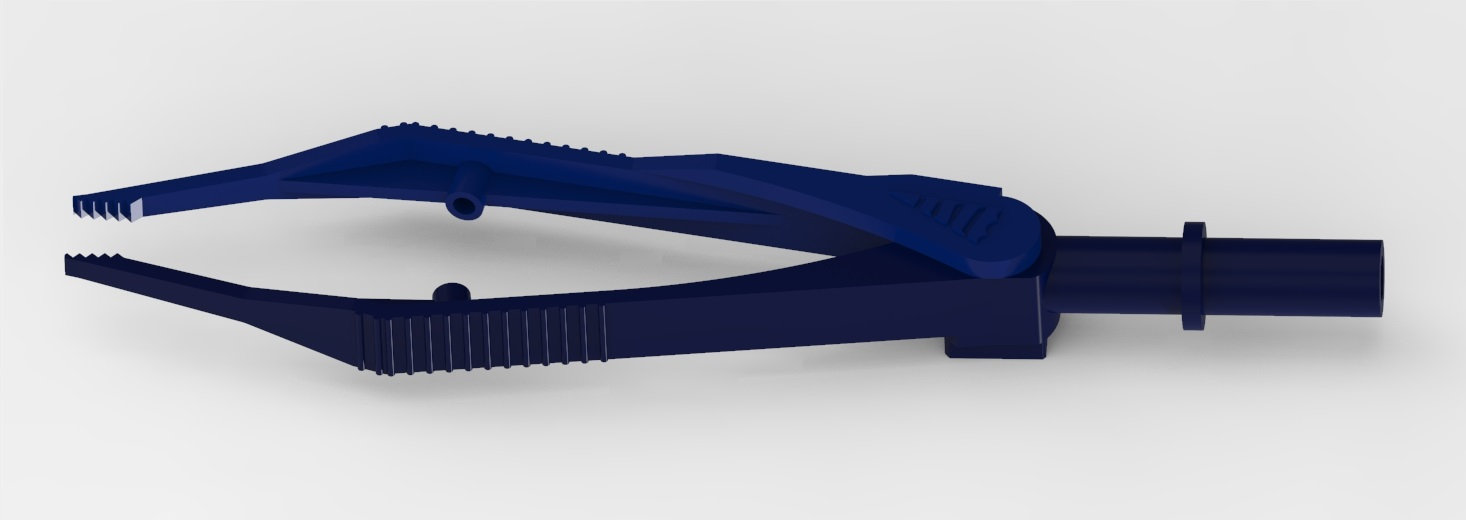
\includegraphics[width=80mm, keepaspectratio]{figures/Szakdoga/csipesz}
\caption{Szakdolgozatomban elkészített telemanipulátorhoz tartozó csipesz\cite{szakdoga}}
\label{fig:Szakdoga_csipeszes}
\end{figure}

A diploma dolgozatom címében megfogalmazott sebészeti eszközök figyelembe vannak véve a bemutatásra kerülő telemanipulátor tervezése közben. A jelző a sebészeti eszközökre szakdolgozatomtól eltérően nem konkrétan a telemanipulátor end-effektorára vonatkozik, hanem a robotkar hatodik csuklójára helyezett eszközre, amit majd a későbbiekben könnyedén lehet ezzel az eszközzel vezérelni.

\begin{figure}[!ht]
\centering
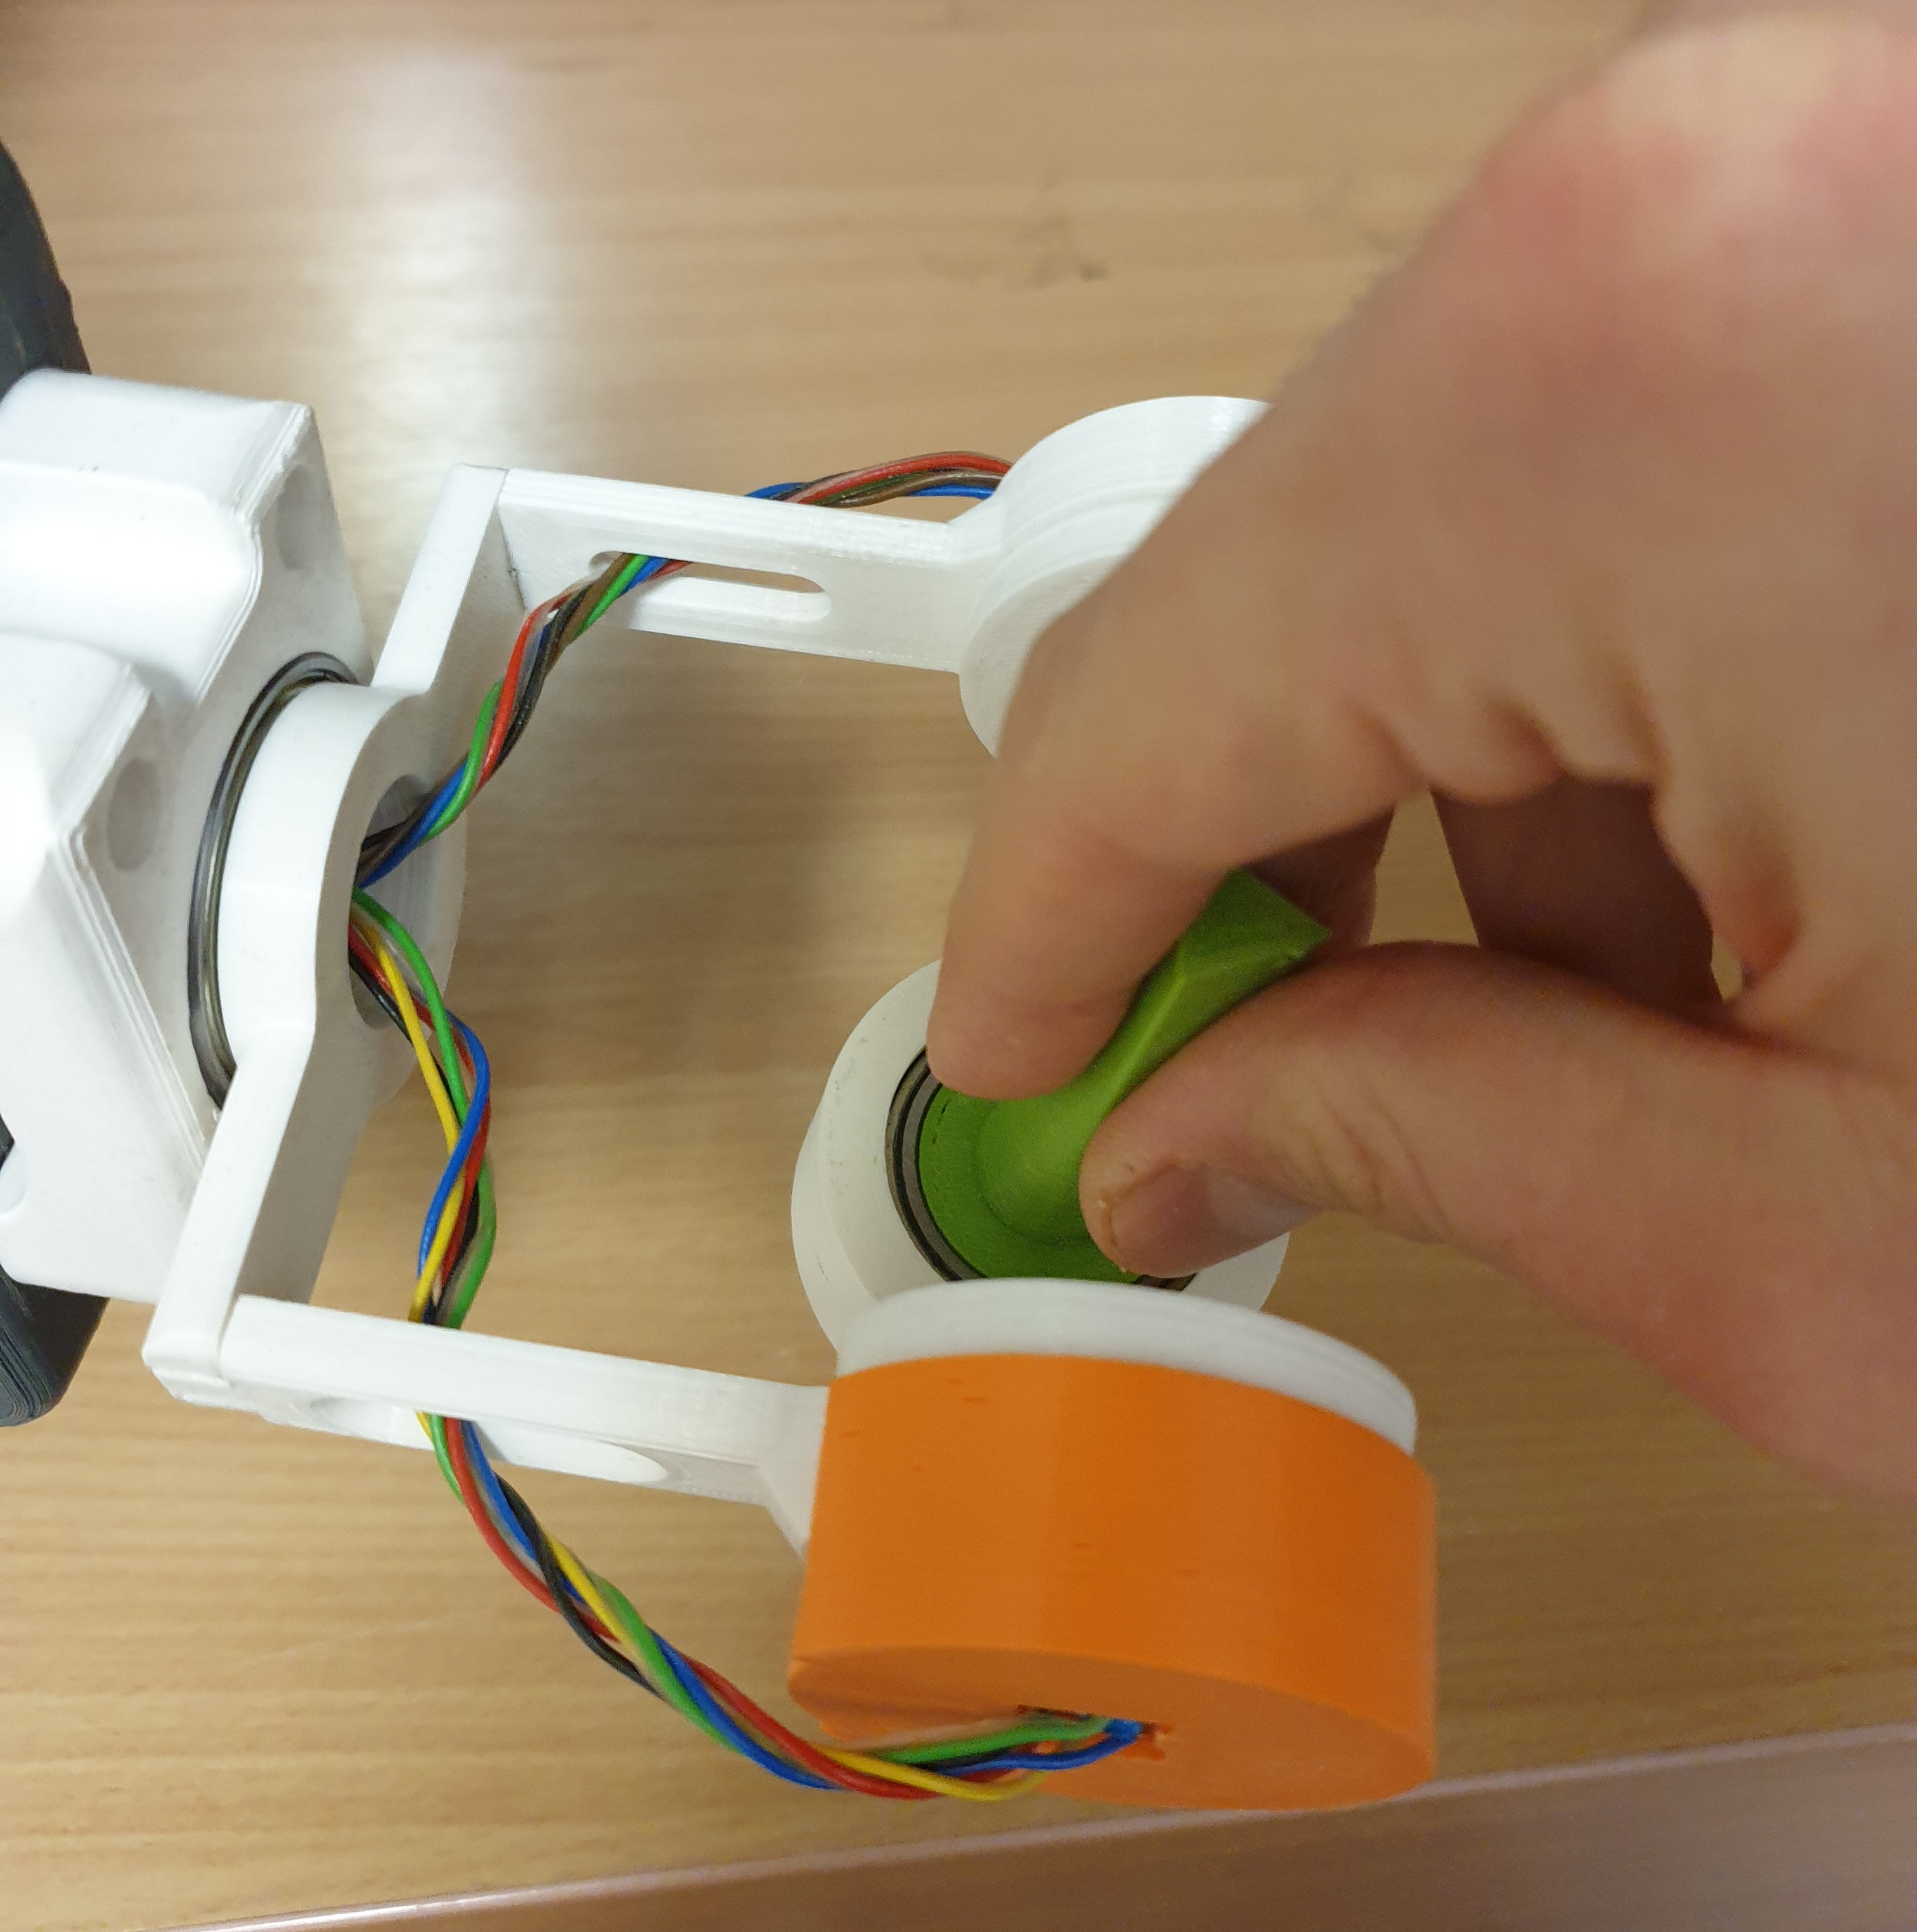
\includegraphics[width=80mm, keepaspectratio]{figures/Szumma/Megfogott_megfogo}
\caption{Diploma dolgozatomban elkészített telemanipulátorhoz tartozó megfogó}
\label{fig:Diploma_EE}
\end{figure}